\section{Design Evaluation}
\label{sec:theory}

\subsection{Design Load Cases (DLCs)}
The user must specify the metocean conditions that drive the wind and
wave loads upon the floating substructure.  \textit{FloatingSE}
currently only uses the single load case of maximum thrust coincident
with maximum wave loading to drive the substructure design. Ideally,
multiple DLCs and metocean conditions would be used for design
optimization.  The capability to optimize over multiple DLCs will be
added to future versions of the model.

\subsection{Load Path}
As with other WISDEM models, the primary simplification in
\textit{FloatingSE} is the treatment of all loads as pseudo-static. This
approximation reduces computational time and resources, since an
accurate calculation of dynamic loads requires more sophisticated
numerical tools and simulations.  Thus, users must exercise care in
selecting loads and safety factors to compensate for the lack of a fully
dynamic treatment \citep{damiani2016}.  Furthermore, fatigue effects and
structural lifetime estimates are also excluded for now, but could be
incorporated in future developments.

A floating wind turbine undergoes loading from a number of sources.  The
primary loading source for the tower comes from the aerodynamic loads
induced by the rotor. The substructure must resist the combination of
both rotor loads and hydrodynamics loads, with the latter becoming more
and more important as water depth and wave heights increase.
\textit{FloatingSE}, together with other WISDEM modules, accounts for
these two dominant load sources, as well as the self-loading of gravity
loads.  Other sources of loading, such as installation loads, accidental
loads, vortex-induced vibrations, ice, and seismic loads are ignored.

\subsubsection{Wind and Wave Loads}
Wind drag loads are applied to the tower body and the upper part of the
substructure that extends above the waterline.  They are not applied to
connecting truss members that may be part of the substructure geometry.
These drag loads are computed assuming the tower and columns are smooth
circular cross-sections and that the drag coefficient can be selected as
a function of the flow Reynolds number \citep{Roshko}.  The drag force
is a function height, since the wind profile and cross-sectional geometry varies
along that dimension.  For the wind profile, the standard power-law
scaling is used,
\begin{equation}
  U_a(z) = U_{ref}\left(\frac{z}{z_{ref}}\right)^{\alpha}\quad,
\end{equation}
where $U_a(z)$ is the wind velocity as a function of height, $U_{ref}$ is a
reference wind speed measured at a reference height, $z_{ref}$, and
$\alpha$ is the shear exponent used in the power-law approximation of
wind profiles.  The wind profile then feeds the aerodynamic drag,
Reynolds number, and drag coefficient,
\begin{equation} \label{eqn:drag}
  dF(z) = \frac{1}{2} \rho_a U_a^2(z) d(z) c_d(Re) dz;\qquad
  Re_d = \frac{\rho_a U_a(z) d(z)}{\mu_a}\quad,
\end{equation}
where $Re_d$ is the Reynolds number based on diameter, $\rho_a$ and
$\mu_a$ are the density and viscosity of air, $d(z)$ is the diameter of
the column as a function of height, $c_d$ is the 2-D drag coefficient, and
$dF(z)$ is the force per unit length in the z-direction.

Wave drag loads arise from similar processes, but are computed using
Morison's equation, a semi-empirical expression that predicts the total
hydrodynamic loads.  It is comprised of two components, one for viscous
drag contributions and another for inertial effects (which includes
incident, diffracted, and radiated wave effects).  For flow past
structures with circular cross sections, Morison's equation for force
per unit length ($dF(z)$) takes the form,
\begin{equation} \label{eqn:morison}
  dF(z) = \frac{\pi d^2(z)}{4} \rho_w C_m \dot{U}_w(z)dz + \frac{1}{2} \rho_w U_w^2(z) d(z) c_d(Re)dz\quad,
\end{equation}
where $C_m$ is the added mass coefficient (assumed to be $C_m=2$),
$U_w(z)$ is the current speed as a function of height, $\dot{U}_w(z)$ is
the acceleration as a function of height, and the Reynolds number is
computed by substituting in the appropriate properties for water,
\begin{equation}
Re_d = \frac{\rho_w U_w(z) d(z)}{\mu_w}\quad.
\end{equation}

To compute Morison's equation, expressions for local fluid velocity and
acceleration are required.  Wave particle velocity (not the same as the bulk
velocity of the wave) is assumed to follow linear (Airy) wave theory
\begin{equation} \label{eqn:Uwave}
U_w(z) = a\omega\frac{\cosh\left[\kappa\left(z + D \right)\right]}{\sinh\left(\kappa D\right)}\cosh\left(\kappa x -
  \omega t\right);
\qquad \omega=\frac{2\pi}{T} = \sqrt{ g \kappa \tanh\left(\kappa
    D\right) } \quad,
\end{equation}
where $\omega$ is the circular frequency, $T$ is the wave period, $a$ is
the wave amplitude (half of the significant wave height), $D$ is the
total water depth, $g$ is the acceleration of gravity, and $\kappa$ is
the wave number numerically computed from the dispersion relationship
given as the last expression in Equation \ref{eqn:Uwave}.  Note that the
horizontal particle velocity varies in time and space (by the
$\kappa x - \omega t$) term.  Thus, the individual particles in the wave
are also accelerating at different rates,
\begin{equation} \label{eqn:Awave}
\dot{U}_w(z) = a\omega^2\frac{\cosh\left[\kappa\left(z + D \right)\right]}{\sinh\left(\kappa D\right)}\sinh\left(\kappa x -
  \omega t\right)\quad.
\end{equation}
For
simplicity, \textit{FloatingSE} only considers the maximum velocity and
acceleration at a given height, and makes a conservative assumption that
they occur concurrently in time and space.  This essentially means ignoring the
$\kappa x - \omega t$ term, since the maximum of any hyperbolic sine or cosine
term is one.


\subsubsection{Rotor Nacelle Assembly (RNA) Loads}
From a quasi-steady-state point of view, the RNA loads reduce to three
forces and three moments along the main coordinate axes
\citep{JacketSE}. The thrust is the biggest force responsible for the
bending moment distribution along the tower and loads on the
substructure.  There is the additional effect of the gravitational load
caused by the offset of the RNA center of mass from the tower
centerline.  This effect is more pronounced for downwind turbines than
upwind turbines, but is included regardless.  \textit{FloatingSE} does
not compute the force and moment components directly, but rather accepts
them as inputs from other WISDEM modules or from the user directly.


\subsection{Structural Analysis}
The analysis tool, Frame3DD, is an open-source tool for static and
dynamic structural analysis of 2-D and 3-D frames and trusses with
elastic and geometric stiffness. It computes the static deflections,
reactions, internal element forces, natural frequencies, and modal
shapes using direct stiffness and mass assembly \citep{frame3dd}.  The
WISDEM toolkit developed a python interface, \textit{pyFrame3DD}, to
avoid the use of intermediate input and output text files.  The
integration of all loads happens within Frame3DD, where the whole floating
turbine load path, from the rotor to the keel of the substructure, is
modeled with Timoshenko frame elements \citep{timoshenko}.

\subsubsection{Discretization}
For the finite element structural analysis of the substructure, the
discretization of the main columns into a handful of sections is still
too coarse to capture the appropriate physics. Long slender components,
such as the tower and substructure columns, are broken up into a
three-times finer discretization than the physical cans that they are
actually made of.  The sectional and nodal variables are re-sampled at
this finer spacing.  These additional discretization points give greater
resolution of internal forces and natural frequencies.  Substructure
pontoons are represented as single frame elements.  Frame elements are
described by their cross sectional properties (area, moments of inertia,
modulus of elasticity, and mass density) and starting and ending nodes.
For simple geometries, such as pontoons with tubular cross sections,
these properties are straightforward calculations.  For the turbine
tower, tubular cross section properties are also used, albeit at a finer
discretization.  For substructure columns, it is assumed that the
permanent or variable ballast and bulkheads are not load-bearing, so
tubular cross section properties are also used to represent the column
shell.  However, the material mass density of the frame element is
scaled to reflect the true mass of the whole section, including ballast,
to ensure that gravity loads are captured correctly.

\subsubsection{Loads}
All of the loads described above are integrated together within
Frame3DD.  These loads include,
\begin{itemize}
\item Rotor-nacelle-assembly loads (thrust, moments, etc)
\item Mooring line force
\item Wind and wave loading
\item Gravity loads (weight distribution)
\item Hydrostatic pressure loads, including buoyancy
\end{itemize}

The forces, moments, and mass properties of the rotor-nacelle assembly
(RNA) are inputs to \textit{FloatingSE} (mass properties are assumed to
be relative to the tower top position).  It assumed that the RNA is a
rigid body with respect to the tower modes and the mass properties,
forces, and moments, are applied to the corresponding node in the model.
The forces along each mooring line are applied to the connection
point nodes on the structure.  The wind and wave forces per unit length
in Equations \ref{eqn:drag} and \ref{eqn:morison} are applied as
trapezoidally varying loads along the column elements.  Other loads
applied to the structure include the gravity loads, and the buoyancy
acting on the submerged elements.

\subsubsection{Boundary Conditions}
Multiple boundary conditions are applied to the structure.  The mooring
system stiffness matrix (linearized about the neutral position) is
applied at the mooring connection nodes.  However, even with the mooring
stiffness, the finite element analysis would otherwise still regard the
structure as unrestrained and incapable of supporting any static loads.
Thus, in order to successfully compute stress and buckling limits in a
well-posed problem, an additional rigid boundary condition (in all 6
DOF) is imposed at the bottom node of the main column.

\subsubsection{Outputs}
Structural analysis outputs include mass properties of the structure,
member stresses, and summary forces and moments on the body.  Mass
properties include the total mass of the floating turbine and the mass
of the substructure itself.  The calculations also allow for easy
computation of the center of mass of the structure (not accounting for
variable ballast) and the center of buoyancy (centroid of the submerged
volume).  The first two natural frequencies of the structure are also
computed to compare against the range of standard wave frequencies and
rotor passing frequencies (1P and 3P).  Next, the reaction forces and
moments at the boundary node at the keel are taken as the total loading
on the structure.  These are used later in the static stability
calculations to ensure that the mooring lines provide adequate restoring
force and moment.  Finally, the axial and shear forces within each frame
element are extracted and converted to stresses using cross-sectional
properties.

Hoop stress of the tower is estimated from the dynamic pressure of the
wind loads using the Eurocode method \citep{Eurocode}.  Hoop stress of the submerged
columns is determined using the dynamic and static pressure heads of the
water.
\begin{align}
  \sigma_{\theta,Euro} &= k_w q_{max} \frac{d-t}{2t};\qquad q_{max} =
                         \frac{1}{2}\rho_a U_a^2\\
  \sigma_{\theta,hydro} &= \left(q_{max}+p_{hydro}\right) \frac{d-t}{2t};\qquad q_{max} =
                          \frac{1}{2}\rho_w U_w^2\\
  p_{hydro} &= \rho_w g \left( a\frac{\cosh\left[\kappa\left(z + D \right)\right]}{\cosh\left(\kappa D\right)} - z\right)
\end{align}
where $\sigma_{\theta}$ is the hoop stress, $q_{max}$ is the maximum
dynamic pressure on a cross-section, and $p_{hydro}$ is the hydrostatic
pressure with contributions from wave motion and the static head.  In
the Eurocode method, $k_w$ is the dynamic pressure factor for hoop
stress calculation using cylinder dimensions and an external pressure
buckling factor.  Note that the argument, $(z)$, was dropped from many
of the terms without losing generality.



\subsubsection{Code Compliance as Utilizations}
Once the stress components of all structural members are computed, they
are compared against design code standards for compliance, and serve as
design constraints when conducting optimization.  Multiple code
standards are used across all components.  For all columns, the tower,
and substructure pontoons, stress components (axial, shear, and hoop)
are combined into a von Mises, equivalent, stress,
\begin{equation}
  \sigma_{vm} = \sqrt{\sigma_a^2 + \sigma_{\theta}^2 -
    \sigma_a\sigma_{\theta} + 3\tau_{a\theta}^2}
\end{equation}
where $\sigma_{vm}$ is the von Mises stress, $\sigma_a$ is the axial
stress, $\tau_{a\theta}$ is the shear stress across axial and hoop
principle directions.  and $\sigma_{\theta}$ is chosen as the relevant
hoop stress.  The von Mises stress is compared against the yield stress,
$\sigma_y$, and a safety factor as a utilization criterion.

Main column, offset column, and tower segment stresses and geometry are
also evaluated against a shell buckling criterion published by
\citet{Eurocode} and a global buckling criterion published by
\citet{Germanischer}.  Note that the implementation of the Eurocode
buckling is modified slightly so as to produce continuously
differentiable output.  See \citet{JacketSE} for a more detailed
exposition.

For submerged columns, additional code standard utilization ratios are
taken from the \citet{api2U}, Bulletin 2U (specifically the procedure
outlined in Appendix B).  These standards also apply shell and general
buckling criterion with a margin of safety in a manner that accounts for
stiffeners and the common buckling modes of submerged structures.
Future efforts will also apply Bulletin 2V, the standards for plates, to
the legs that support taut mooring lines.


\subsection{Mooring Lines}
The quasi-steady mooring system analysis is handled by the external
Mooring Analysis Program (MAP++) library \citep{MAP}, which has
convenient Python bindings to access the simulation output, bundled into
the WISDEM \textit{pyMAP} module. MAP++ is designed to model the
steady-state forces on a Multi-Segmented, Quasi-Static (MSQS) mooring
line. Seabed contact, seabed friction, and multi-element mooring lines
with arbitrary connection configurations can be analyzed.  MAP++ inputs
include sea depth, geometry descriptions of the mooring line
connections, and material properties of the lines.  For chain and
rope-based cables, these material properties are not easily derived and
would be typically provided by a manufacturer.  We borrow from the
approach of the popular Orcina OrcaFlex software \citep{orca} and use
the following expressions,
\begin{align*}
MBL &= 2.74\times 10^7  d^2 \left(44 - 80d\right) \,[\unit{N}] \\
mass &= 19.9\times 10^3 d^2 \,[\unit{kg/m}]\\
A &= 2\left(\pi d^2 / 4 \right)\,[\unit{m^2}]\\
EA &= 8.54\times 10^{10} d^2\,[\unit{N}]\\
cost &= 3.415\times 10^4 d^2 \,[\unit{USD}]
\end{align*}
where $MBL$ is minimum breaking load, $d$ is the diameter of a single
half-chain link, $A$ is the chain cross-sectional area, $E$ is the
Young's modulus, $EA$ is the axial stiffness.  When conducting
optimization, the expression for $MBL$ is poorly posed due to its limited
range of diameter applicability, so a linear fit is used instead,
\begin{equation}
MBL = 1000 \max\left(1.0, -5445.3 + 176972.7 d\right)
\end{equation}  


\subsection{Hydrostatic Stability}
\label{sec:static}
\subsubsection{Neutral Buoyancy}
Any floating body requires enough water displacement to create
sufficient buoyancy force such that the body stays afloat in the most
extreme loading and environmental conditions.  This level of
displacement would otherwise be overkill for more benign loading
conditions.  Since a floating turbine is designed for a constant hub
height, variable amounts of ballast are required to maintain a neutrally
buoyant system for all operating conditions.  The variable ballast is
simply ocean water that is pulled in or pumped out of holding areas
within the substructure columns.

In \textit{FloatingSE}, the variable ballast water mass is calculated as
the difference between the total mass of displaced water and the total
mass of the floating turbine.  This mass is then divided by the water
density to obtain the variable ballast volume, which is then compared to
the frustum shell cross section profile above the permanent ballast to
determine the height of the water ballast within the column.  Once this
is determined, the final center of mass of the system can be determined.

\subsubsection{Surge/Sway Stability}
Surge and sway stability is not actively tracked over the coarse of a
load case.  Instead the total surge force on the structure is calculated
at the initial conditions and compared to the restoring force of the
mooring system at the maximum allowable surge offset, which is specified
by the user.

The surge direction is assumed to be aligned with the wind vector, which
is aligned with the $x$-axis.  Since the rotor yaw is assumed to be
$0^{\circ}$, the surge forces on the turbine include the rotor thrust
and the wind and wave drag on the tower and substructure.  The final
surge force over the whole structure is taken from the $x$-direction
reaction force of the reaction node in Frame3DD.

The restoring force is calculated as the smallest possible restoring
force after a displacement in any angular direction in the mooring
model.  Since the alignment of the mooring lines relative to the
incoming wind direction is arbitrary, a maximum offset is simulated at
$2^{\circ}$ increments around the unit circle. Also recorded in this
survey is the maximum mooring line tension in any
line, in any direction, for comparison against the minimum breaking load
value,
\begin{equation}
  F_{x,restore} = \min_{i\in a} F_{x,i}\quad \mbb{T}_{moor} = \max_{l\in L,i\in a} \mbb{T}_{l,i}\,;
\qquad L=\left\{1,2\ldots nlines\right\}, \, a= \left\{0^{\circ}, 2^{\circ}\ldots 360^{\circ}\right\}
\end{equation}
where $F_x$ is the surge force and $\mbb{T}$ is the tension.  If
restoring force at this maximum offset is greater than the surge force
applied, then the system is considered stable in surge.  Since the wind
and wave profiles are essentially 2-D in the $x-z$ plane, the sway
stability is given the same status as surge stability.


\subsubsection{Pitch Stability}
The approach to pitch stability determination is similar to that of
surge stability.  The total pitching moment on the floating turbine is
calculated and compared to the restoring moment at the maximum allowable
angle of heel.  If the restoring moment at this max heel angle is
greater than the pitching moment applied, the system is said to be
statically stable in pitch.

Similar to the surge force calculation, the total pitching moment is
determined from the reaction moment at the boundary condition
in the Frame3DD analysis.  The pitching moment has contributions from
the wind and wave loads on the structure, the rotor forces and torques,
the buoyancy forces on the submerged substructure, and the off-center
weight of components (e.g. the RNA).

The restoring pitching moment has two primary contributions.  The first
is from the mooring lines.  Similar to the surge force calculation, here
the floating turbine is deflected in pitch by the maximum allowable heel
angle and the mooring forces are recorded.  The restoring moment
contribution from the mooring system is computed as,
\begin{equation}
  \mbf{M_{moor}} = \sum_i \mbf{r_{cm-l}} \times \mbf{F_l}
\end{equation}
where $r_{cm-l}$ is the vector from the center of mass to the mooring
connection, and $F_l$ is the force applied by the $l$-\th\~mooring
line.  As above, $F_l$ is taken as the minimum set over the possible
orientations of the mooring lines relative to the direction.

\begin{figure}[htb]
  \begin{subfigure}[b]{0.49\linewidth}
    \centering 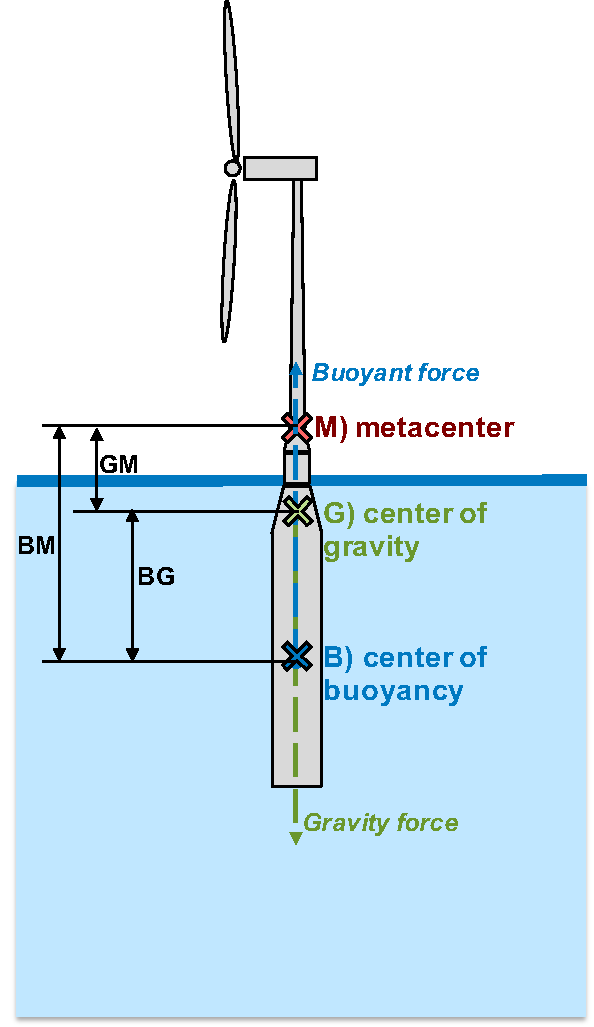
\includegraphics[height=3.5in]{figs/metacenterA.pdf}
    \caption{}
  \end{subfigure}
  \begin{subfigure}[b]{0.49\linewidth}
    \centering 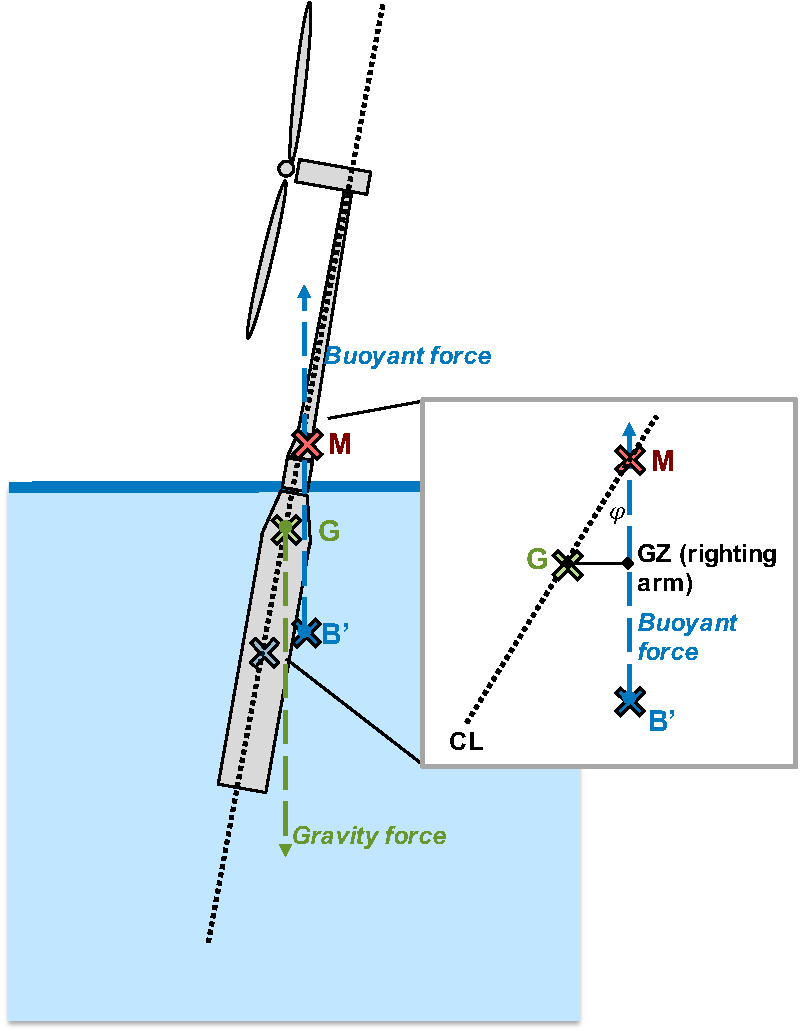
\includegraphics[height=3.5in]{figs/metacenterB.pdf}
    \caption{}
  \end{subfigure}\\
  \caption{Static stability of floating offshore wind turbines.}
  \label{fig:metacenter}
\end{figure}

The second contributing restoring moment comes from the motion of the
center of buoyancy away from alignment with the center of mass.  This is
a standard calculation in naval architecture \citep{thiagarajan2014} and is
diagrammed in Figure \ref{fig:metacenter}.  In this diagram, the center
of mass is denoted, $G$, the center of buoyancy is $B$, and the
metacenter is $M$.  In neural conditions (Figure \ref{fig:metacenter}a),
all of these points are vertically aligned.

As the structure lists or heels, the center of buoyancy shifts toward
the side of the structure that is more submerged (from $B$ to $B'$) and
the buoyancy force no longer passes through the center of mass.
Instead, the buoyancy force passes through the metacenter with an
effective moment arm of $GZ$ from the center of mass (Figure
\ref{fig:metacenter}b).  The metacenter is defined as the common point
through which the buoyancy force acts as it pitches through small
displacements, for bodies with sufficient freeboard margin.

The metacenteric height, $GM$ is most easily calculated as an offset from the
center of buoyancy ($BM$) by,
\begin{equation}
  h_{meta} = M - G = GM = BM + BG;\quad BM = \frac{I_w}{V}
\end{equation}
where $BG$, the distance between the centers of buoyancy and gravity is
easily calculated, $I_w$ is the second moment of area of the substructure waterplane
(with units of \unit{$m^4$}) and $V$ is the total volume of displacement
(with units of \unit{$m^3$}).  Note that for semisubmersible type
geometries, $I_w$ is calculated with the parallel axis theorem for all
of the columns at the waterplane,
\begin{equation}
  I_w = \sum_i \left( I_{w,i} + S_ir_i^2 \right)
\end{equation}
where $S_i$ is the waterplane cross sectional area of the $i$-\th column and $r_i$
is the distance from the waterplane centroid to the $i$-\th column centroid.

The restoring moment is then the buoyancy force acting through the
restoring arm, $GZ$,
\begin{equation}
  M_{meta} = F_B GZ = F_B GM \sin \varphi
\end{equation}
where $\varphi$ is the angle of heel.

For this reason, the metacenter must be located above the center of mass
for static stability.  This condition is imposed on the design as a
constraint.  Note that the total volume of displacement, and the
subsequent buoyancy force, is not recalculated in the perturbed
configuration.  It is assumed that the angles of deflection are small
and that there is sufficient freeboard and design symmetry such that the
total displacement is constant.

The total restoring pitching moment is then the sum of two
contributions,
\begin{equation}
  M_{y,restore} = M_{y,moor} + M_{meta}
\end{equation}

\subsection{Hydrodynamic Stability}
Floating bodies are typically modeled, for small motions and linearized
behavior, as a second-order differential system with mass, damping, and
spring stiffness terms,
\begin{equation}
  \left(\mbf{M} + \mbf{A}\right)\ddot{\mbf{x}} + \mbf{C}\dot{\mbf{x}} +
  \mbf{K} = \mbf{F}\left( t \right)
\end{equation}
where $\mbf{x}\in\mbb{R}^6$ is the six-degree of freedom vector
(commonly ordered as 1-surge, 2-sway, 3-heave, 4-roll, 5-pitch,
6-yaw), $\mbf{M}$ is the mass matrix, $\mbf{A}$ is the added mass
matrix, $\mbf{C}$ is the damping matrix, and $\mbf{K}$ is the stiffness
matrix.  The right-hand side of the equation captures the time-dependent
summation of all forces.

As a low-fidelity, quasi-static sizing and cost module,
\textit{FloatingSE} does not attempt to capture all of the matrix
entries or forcing terms of the hydrodynamics.  A more sophisticated
time- or frequency-domain solver, where these quantities are calculated,
may be linked or included into \textit{FloatingSE} in the future.
Nevertheless, it does attempt to compute the diagonal entries of the
mass and stiffness matrices in order to derive the rigid body natural
frequencies of the system,
\begin{equation}
  f_i = \frac{\omega_i}{2\pi} =
  \frac{1}{2\pi}\sqrt{\frac{K_{ii}}{M_{ii}+A_{ii}}}, \quad \forall i \in
  \left[1\ldots6\right]
\end{equation}
where $f_i$ are the frequencies of the eigenmodes and $\omega_i$ is the
circular frequency.  The mass matrix diagonal entries, $M_{ii}$, are simply the mass and
moments of inertia of the whole system,
\begin{equation}
  M_{11} = M_{22} = M_{33} = m_{sys};\quad M_{44} = I_{xx,sys};\quad M_{55} = I_{yy,sys};\quad M_{66} = I_{zz,sys};
\end{equation}
Where the coordinate system notation is consistent with that of Figure
\ref{fig:diagram}.

The added mass matrix diagonal entries are evaluated via standard strip
theory for the tapered vertical columns.  The added mass for the system is a
summation over the columns, using the parallel axis theorem for the
rotational degrees of freedom.  Pontoon contributions to system added
mass are currently ignored.  The column quantities are calculated as,
\begin{equation}
  A_{11} = A_{22} = \rho V;\quad A_{33} = 
  \left(\frac{1}{2}\right)\frac{8}{3} \rho \max \left[ R^3(z)\right] ; \quad A_{44} =
  A_{55} = \pi\rho\int\left(z-z_{cb}\right)R^2(z)dz;\quad A_{66} = 0.0;
\end{equation}
where $\rho$ is the water density, $R(z)$ is the column radius along its
axis, and $V$ is the submerged volume.  The extra factor of $1/2$ in
$A_{33}$ is included to account for the fact that the top of the column
extends above the waterline.  Also, the integral in $A_{55}$ is only evaluated
along the submerged portion of the column.

The stiffness matrix is comprised of contributions from the mooring
and hydrostatic stiffness.  The mooring linearized stiffness matrix is output
directly from MAP++ and needs no additional processing within
\textit{FloatingSE}.  The hydrostatic stiffness, for a vertical column, is derived from the same
principals described above regarding the metacentric height,
\begin{equation}
  K_{ii} = K_{ii}^{moor} + K_{ii}^{hydro};\quad K_{33}^{hydro} = \rho g
  S_{sys};\quad K_{44}^{hydro} =  K_{55}^{hydro} = \rho g V h_{meta}
\end{equation}
where $S_{sys}$ is the waterplane area of the system.

Once the rigid body natural frequencies (eigenmodes) of the system are
calculated, they are compared against the standard wave frequencies
range, \unit[0.5--5]{Hz}, and expressed as a design constraint (with a
partial safety factor).


\subsection{Validation}
The International Energy Agency has sponsored a number of international
research collaborations to further the state of wind energy technology and
tools.  One of these, Task 30: Offshore Code Comparison Collaboration
(OC3), shared a spar design among many participants to compare
performance as modeled by differed tool sets.  A description of the OC3
spar is provided in \citet{OC3}.  Since it is already a
well-studied geometry, this design was selected as the focus of
verification for \textit{FloatingSE}.  As part of the Task 30 effort,
an ANSYS model of the OC3 spar, using shell elements combined with
stiffeners and bulkheads, was also generated.  This was taken as
the \textit{truth} standard for comparison.

The first step in the verification exercise was to ensure that the mass
properties of the spar predicted by \textit{FloatingSE} matched those
calculated by ANSYS.  The comparison showed that the \textit{FloatingSE}
summary mass estimates are within $1\%$ error of ANSYS.  The second step
was a comparison of static loading stresses.  The spar was simulated in
quiescent air and water (no wind, waves, or current), which isolated the
weight of the turbine and hydrostatic pressure forces as the only load
sources on the substructure.  The effective von Mises stress, as
calculated by \textit{FloatingSE}, was compared to the ANSYS model.  The
\textit{FloatingSE} stress calculation matches that of ANSYS nearly
exactly over the top half of the spar, but deviates by approximately
5--10\% towards the bottom half of the spar.  In the bottom half of the
spar, \textit{FloatingSE} actually over-predicts the stress, a more
conservative estimate, which is the preferable approach in a
low-fidelity cost and sizing model.  At this time, more complicated
loading cases, with wind and wave loading included, have not been
performed.

The rigid body modes predicted by \textit{FloatingSE} were compared
against a FAST model of the OC3 spar.  FAST was used as the truth
solution in this case because it more accurately handles mooring
dynamics than the ANSYS structural model and more accurately captures
hydrodynamic phenomenon.  The errors in the surge, sway, roll, and pitch
frequencies are 11-12\%.  \textit{FloatingSE} actually estimates the
heave mode frequency quite accurately, to less than 1\% error, but is
significantly off in estimating the yaw mode frequency.  This was deemed
acceptable as there is no focus on the yaw DOF in \textit{FloatingSE}.



